% ##################################################################################################################
\chapter{Yokohama: MATSim Application for Resilient Urban Design}
\label{ch:yokohama}
\hfill \textbf{Authors:} Yoshiki Yamagata, Hajime Seya, Daisuke Murakami

% ##################################################################################################################
\section{Introduction}
In \citet[][]{YamagataSeya_ITSIET_2015}, we proposed the concept of a resilient local electricity-sharing system as a complement, or alternative, to a \gls{fit} to achieve $CO_2$-neutral transportation in cities. In our proposed system, electricity generated from widely introduced solar \glspl{pv}
%\ah{why PV? PhotoVoltaic. But then Panel has to be removed from accronym.} 
is stored in cars ``not in use'' in a city. In Japan, almost half the central Tokyo metropolitan area cars are used only on weekends and thus are kept parked weekdays. These cars could represent a huge new storage potential if they were replaced by \glspl{ev}; that is, they could be used as storage batteries in a \gls{v2c} system. 

This study analyzed the potential of \glspl{ev} as storage batteries in emergency cases. Specifically, we focused on the following three questions: 
\begin{enumerate}\styleEnumerate
\item How much residential demand can be met ( in each 24\,hour) by electricity from just \glspl{pv}, which are installed on the roofs of all detached houses in the study area? 
\item How many \glspl{ev} are needed to store all surplus electricity (\gls{pv} supply minus demand)?
\item How does \glspl{ev} driving change the load curve and how can mass-adopted \glspl{pv} fulfill total demand? 
\end{enumerate}
To answer our second and third questions, we needed to know (a) the number of cars parked at home during each hour (that is, the time each car arrived at home after use) and (b) the amount of battery charge consumed by each driver during his/her daily trips (that is, trip duration). For this simulation, we used \gls{matsim}. In this chapter, we briefly introduce our \gls{matsim} application for a local electricity-sharing system in Yokohama city, based on \citet[][]{YamagataSeya_ApE_2013, YamagataEtAl_EnPro_2014, YamagataEtAl_ICAE_2015}.

% ##################################################################################################################
\section{Results}
We assumed that \gls{pv} was installed on the roof of each detached house in Yokohama city. Then, we calculated the amount of electricity supplied each hour throughout the whole day by employing simple intensity method. 
%Our target period was 2008; the data we gathered are summarized in Table~\ref{tab:yokohama_tab1}.
%\ah{see the email discussion with Yoshiki} 
The \gls{od} trip data used are from the Fourth Person Trip Survey in Tokyo Metropolitan Area, implemented in 1998. The data are available through the People Flow Project (\url{http://pflow.csis.u-tokyo.ac.jp}) on request (application) and include the \gls{od} trips by traffic mode, time of day, purpose, etc. for each micro district, called \emph{cho-cho-moku}. The Person Trip survey is a national survey that focuses on people's travel behavior during a given few days of each month, from October to December. Because the number of cars in Yokohama for each cho-cho-moku was unknown, the city-level value was allocated to the cho-cho-moku (areal weighting) and adjusted for the size of the population. The road-network information was taken from the National Digital Road Map Database and included sufficient data on road capacity, width classification, link length, number of lanes and travel speed to perform traffic simulations in \gls{matsim}. \gls{matsim} requires a daily ``plan file'' for each agent (car driver); we prepared these files by using the Fourth Person Trip Survey, which captured the daily movements of 722\,000 people. Because the Fourth Person Trip Survey sampled approximately 2\,\% of the population of the Tokyo metropolitan area, the plan file was replicated according to the intensity factor provided by the People Flow Project, resulting in 505\,335 agents. From the \gls{matsim} simulation, we had obtained each agent's trip duration and arrival time. 

Considering load curve changes due to the \glspl{ev} driving, we then asked if massively adopted \glspl{pv} would be enough to satisfy total energy demand in Yokohama. In Figure~\ref{fig:yokohama_fig1}, the solid and dashed lines represent electricity surplus cumulative distribution, charged to or discharged from the batteries of \glspl{ev}, not in use and used only for charging the \glspl{ev} in use, during May and August (solid line, maximum; dashed line, average). The dotted line in the figure represents the scenario where electricity surplus was both charging \glspl{ev} and satisfying households' typical electricity demand under maximal/average solar irradiance. However, in August (high demand, high \gls{pv} supply), the electricity surplus was sufficient for charging \glspl{ev}, but not enough to meet the households' huge electricity demand due to evening use of air-conditioning. 
%
 %------------
\createfigure%
{Cumulative distribution of electricity surplus charged to or discharged for electricity demand (y axis denotes the cumulative distribution of electricity surplus)}%
{Cumulative distribution of electricity surplus charged to or discharged for electricity demand (y axis denotes the cumulative distribution of electricity surplus)}%
{\label{fig:yokohama_fig1}}%
{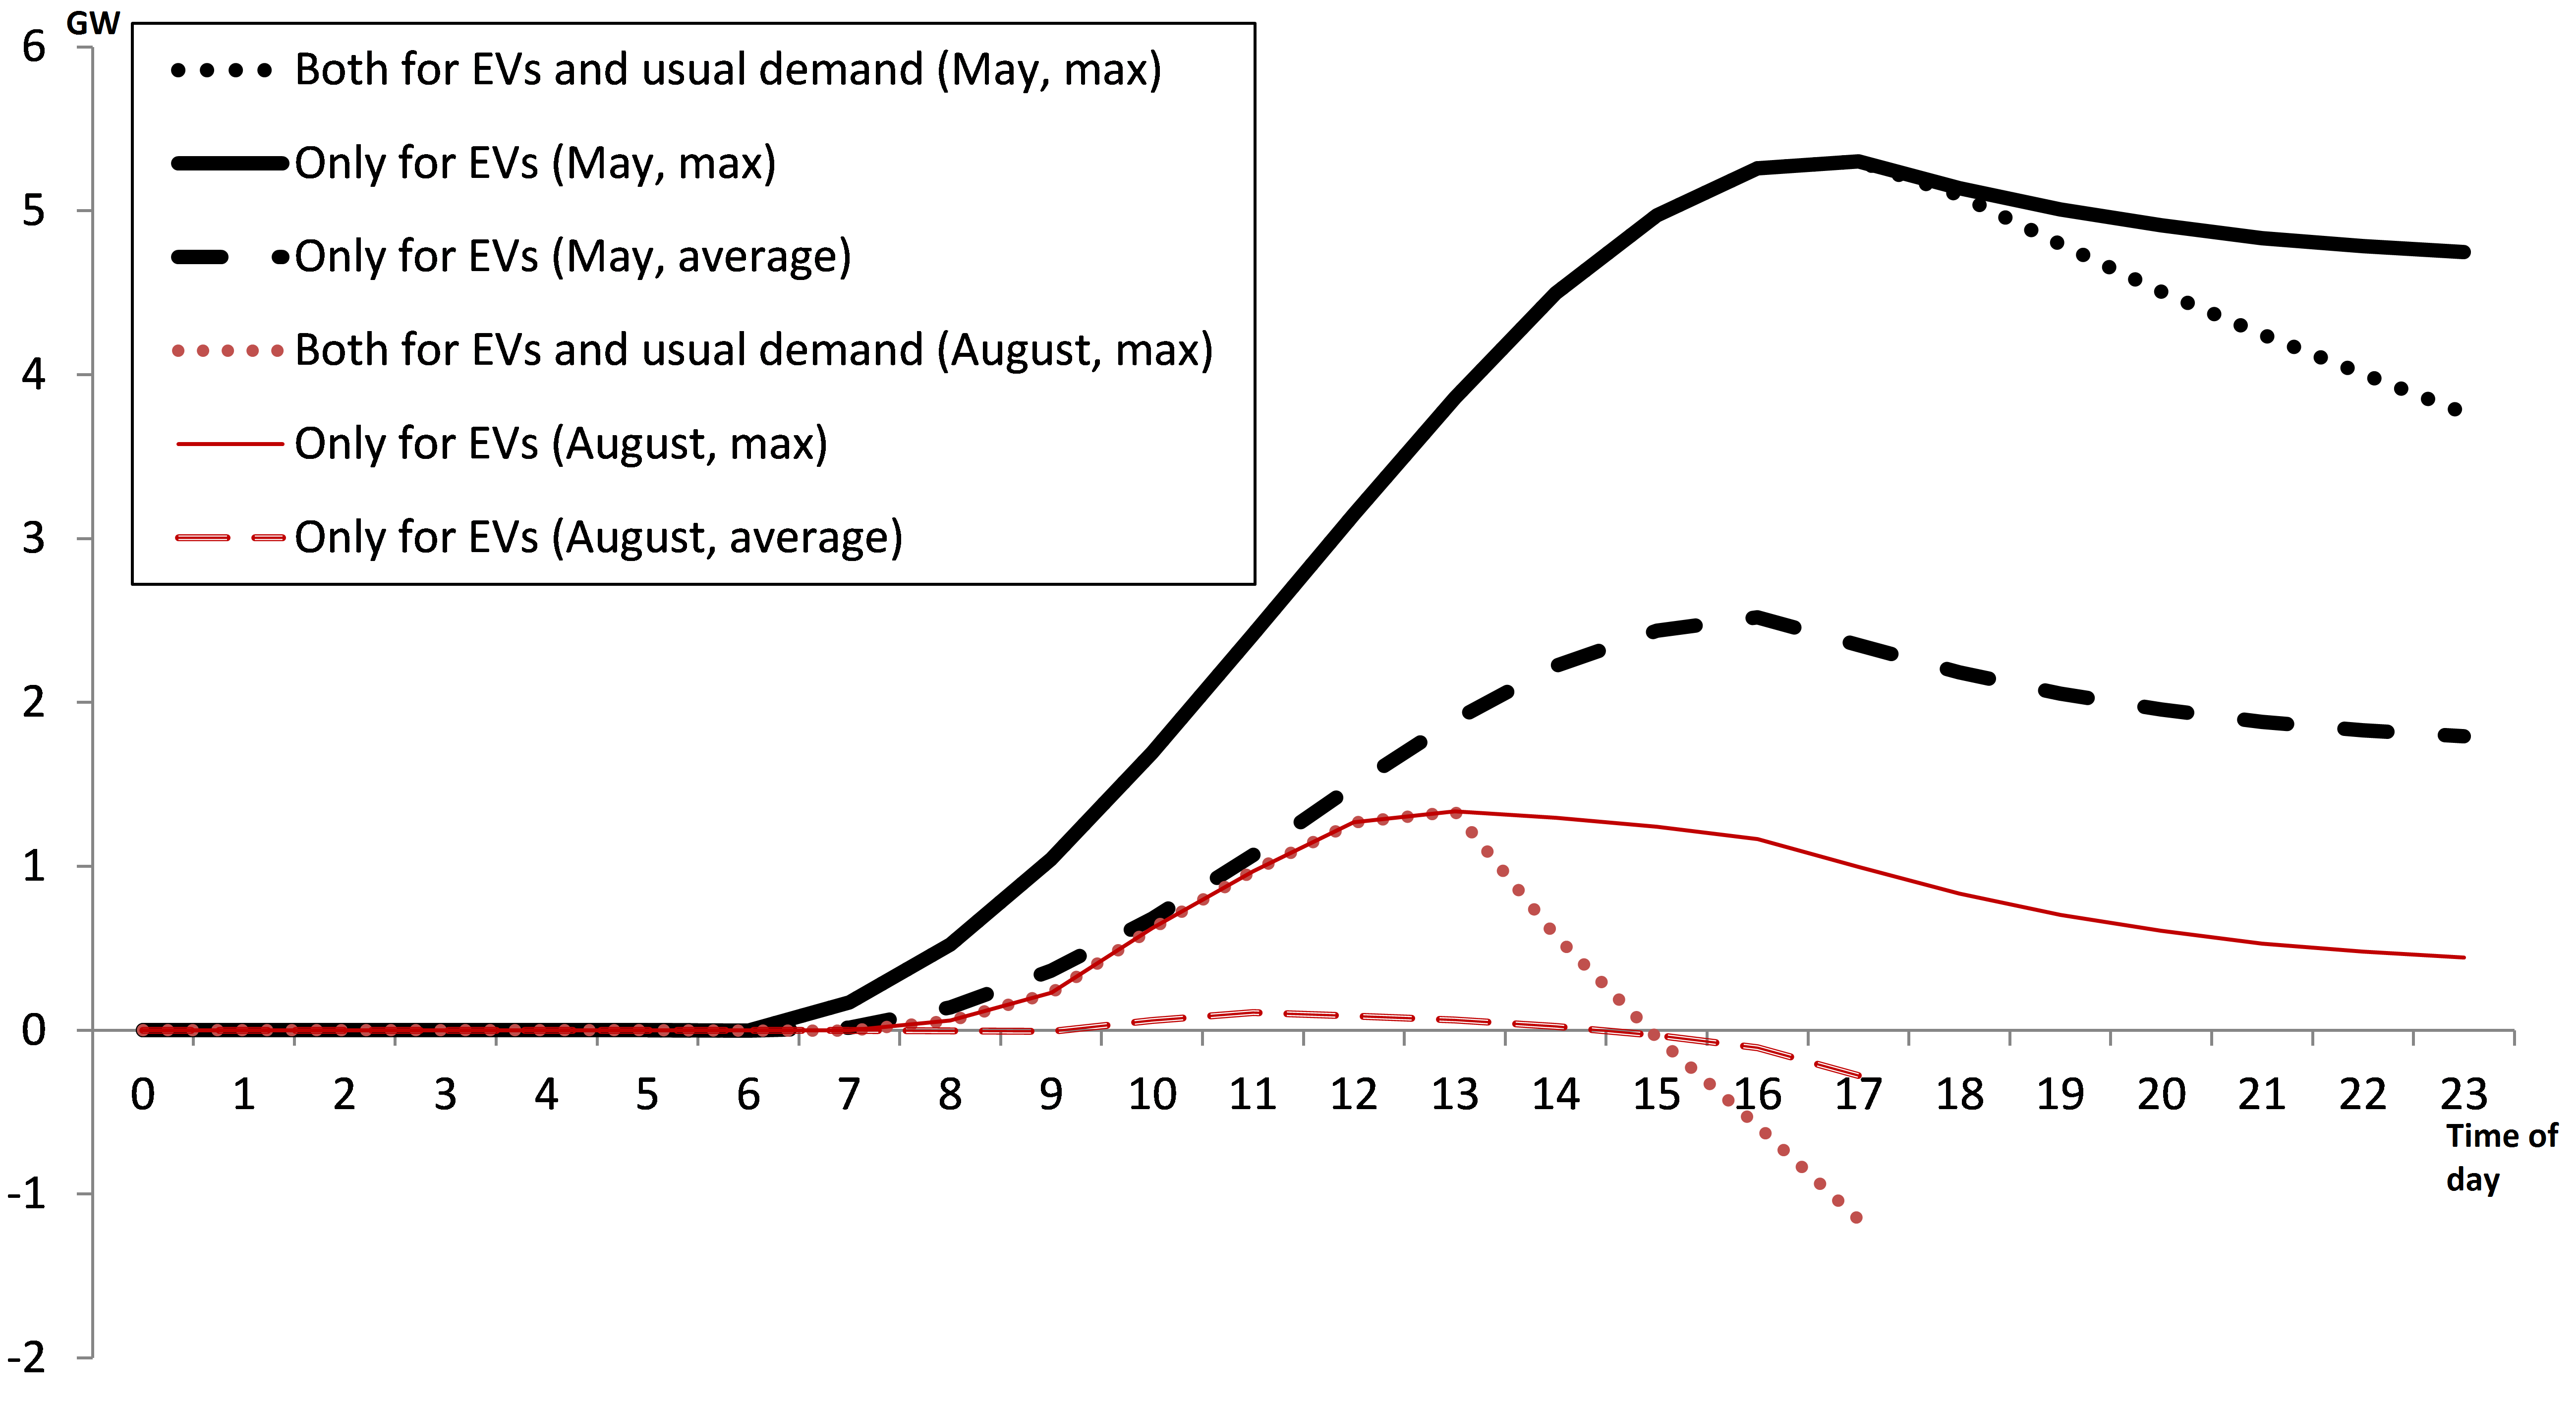
\includegraphics[width=0.85\textwidth, angle=0]{./scenarios/figures/yokohama_fig1.png}}%
{Reproduced by permission of the Institution of Engineering \& Technology: published in \citet[][Figure~6]{YamagataSeya_ITSIET_2015}}
 %------------

To meet household electricity demand, \gls{pv} electricity needs be efficiently stored in \glspl{ev} and locally shared. For example, if a high-affordability zone (storage capacity is greater than electricity surplus) is adjacent to a low-affordability zone (storage capacity is smaller than electricity surplus), then the share of their \gls{ev} capacity increases the ratio of stored \gls{pv} electricity. Because storage affordability (storage capacity minus electricity surplus) is significantly different regionally (see Figure~\ref{fig:yokohama_fig2}), clustering of  community-based local sharing must be carefully designed. In this study, we attempted to optimize community clusters using several different algorithms. Firstly, the number of clusters was assumed 18 to be the same as the number of Yokohama city wards. Then, cluster optimization was performed by minimizing (the sum of storage affordability in the 18\,clusters) plus $k$ (minimum circularity in these clusters), where $k$ was the weight for the circularity. The first term balanced storage capacity and electricity surplus to increases the rate of stored \gls{pv} electricity; the second term decreased inter-point distance within each cluster, as well as electricity sharing (transmission) cost. The minimization was conducted in every month through a simulated annealing algorithm to find optimal spatially clustered communities.
%
 %------------
\createfigure%
{Storage affordability: Storage capacity minus electricity surplus in kWh/day (10\,\% of \glspl{ev} not in use being used as battery)}%
{Storage affordability: Storage capacity minus electricity surplus in kWh/day (10\,\% of \glspl{ev} not in use being used as battery)}%
{\label{fig:yokohama_fig2}}%
{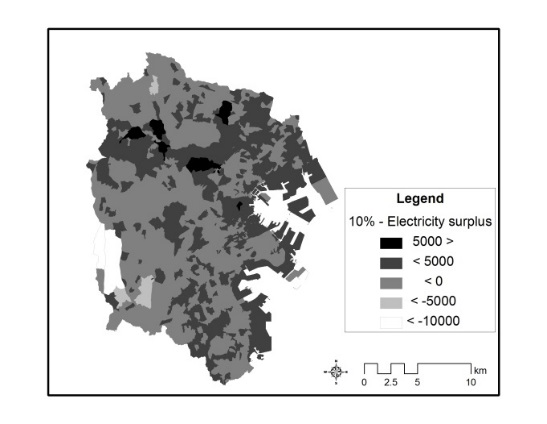
\includegraphics[width=0.85\textwidth, angle=0]{./scenarios/figures/yokohama_fig2.png}}%
{Reproduced by permission of the Institution of Engineering \& Technology: published in \citet[][Figure~10.a]{YamagataSeya_ITSIET_2015}}
 %------------
%
 %------------
\createfigure%
{Monthly clustering results}%
{Monthly clustering results}%
{\label{fig:yokohama_fig3}}%
{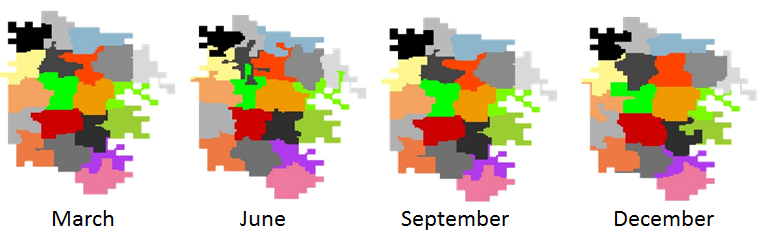
\includegraphics[width=0.7\textwidth, angle=0]{./scenarios/figures/yokohama_fig3.png}}%
{}
 %------------

Figure~\ref{fig:yokohama_fig3} shows four-month clustering results; all clusters indicate positive storage affordability in April, May, June, July, September, and October. In other words, \gls{pv} electricity covers whole household electricity demands, if \gls{ev} capacities are shared with these optimized clusters.

In summary, we applied \gls{matsim} to analyze the potential of \glspl{ev} in a \gls{v2c} system and found that \glspl{ev} can cover typical household electricity demands in some months and the cover ratio can be increased by community clustering for local electricity sharing. In the future study, we plan to use \gls{matsim} to simulate mobility behavior for electricity sharing community scenarios and extend our clustering analysis utilizing simulated behavior. Finally, development of community level mobility sharing service would be a very important topic to integrate \gls{matsim} simulations with our land use and transportation scenarios, such as compact and dispersion scenarios \citep[see][]{YamagataEtAl_AoG_2013}.

% ##################################################################################################################